%----------------------------------------------------------------------------
\appendix
%----------------------------------------------------------------------------
\chapter*{\fuggelek}\addcontentsline{toc}{chapter}{\fuggelek}
\setcounter{chapter}{\appendixnumber}
%\setcounter{equation}{0} % a fofejezet-szamlalo az angol ABC 6. betuje (F) lesz
\numberwithin{equation}{section}
\numberwithin{figure}{section}
\numberwithin{lstlisting}{section}
%\numberwithin{tabular}{section}

\section{Plotting the First 16 Basis Fields}
\label{appendix:first_16}

\begin{figure}[!htb]
  \centering
    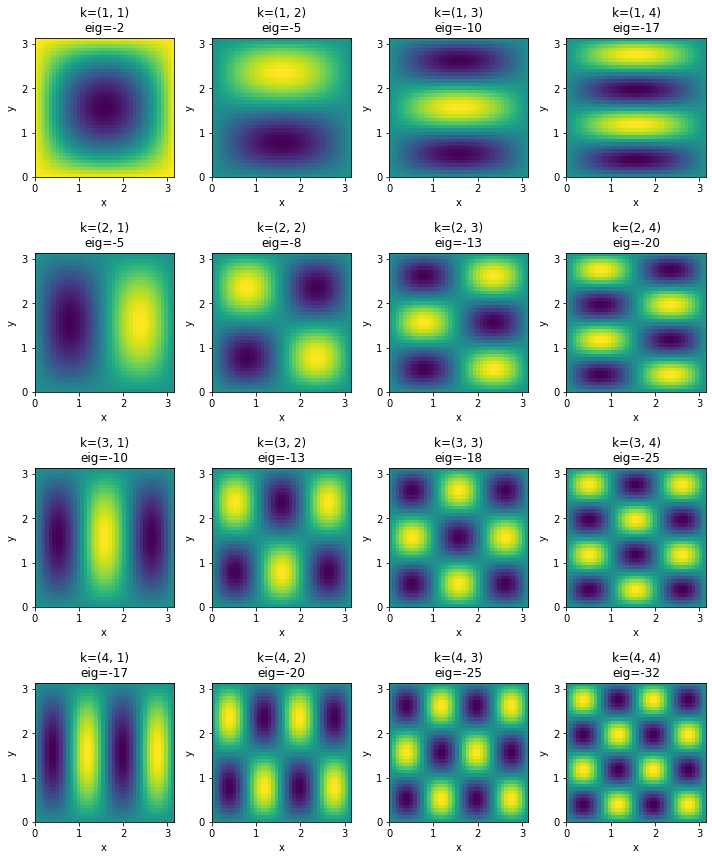
\includegraphics[width=0.9\textwidth]{figures/eigenfluids/16_basis_fields.png}
    \caption{Visualizing the first $16$ $\Phi_{\vb{k}}$ basis fields, sampled on
    a $40 \times 40$ grid in our simulation domain $D = [0,\pi] \times [0,\pi]$.
    Larger magnitudes of eigenvalues correspond to smaller scale
  vortices.}
\end{figure}
